\documentclass[12pt,fleqn]{article}
\setlength{\parindent}{0pt}
\usepackage{graphicx}
\usepackage{cancel}
\usepackage{listings}
\usepackage[latin5]{inputenc}
\usepackage{color}
\setlength{\parskip}{8pt}
\setlength{\parsep}{0pt}
\setlength{\headsep}{0pt}
\setlength{\topskip}{0pt}
\setlength{\topmargin}{0pt}
\setlength{\topsep}{0pt}
\setlength{\partopsep}{0pt}
\setlength{\mathindent}{0cm}
\usepackage{latexsym}
\usepackage{amsfonts}
\usepackage{showkeys}
\renewcommand*\showkeyslabelformat[1]{(#1)}

\begin{document}
Isi Denklemini Turetmek 

Bu denklemi turetmek icin ``enerjinini muhafazasi (conservation of
energy)'' kuralini kullanacagiz. Bu muhafaza kuralini bir esitlige
cevirecegiz, ve bu esitligi manipule ederek ortaya bir kismi turevsel
denklem (PDE) cikaratacagiz. Baz aldigimiz fiziksel ortam bir metal cubuk,
ki bu cubukta materyel yogunlugu her noktada ayni.  Formul soyle;

$[x,x+\Delta x]$ icindeki net isi degisimi = Tanimlanan bolge
sinirlarindaki net isi akisi + $[x,x+\Delta x]$ icinde uretilen isi miktari

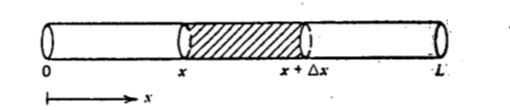
\includegraphics[height=2cm]{heat_1.png}

$[x,x+\Delta x]$ icindeki toplam isiyi nasil hesaplariz? Eger $u(x,t)$
metal cubugun $x$ noktasinda $t$ anindaki isiyi veriyorsa, verilen kesit
uzerinden bir entegral aliriz,

\[ [x,x+\Delta x] \textit{ Icindeki Toplam Isi} = 
cpA \int _{ x}^{x+\Delta x}u(s,t) ds
   \]

Tanimlanan bolge icindeki net isi degimini ise alttaki ile hesaplariz,
ustteki formulun zamana gore turevini aliriz. 


\[ \frac{d}{dt} \int _{ x}^{x+\Delta x} c\rho A u(s,t) ds = 
c\rho A  \int _{ x}^{x+\Delta x} u_t(s,t) ds
  \]


Turevin entegral icine nufuz ettigini goruyoruz, sabit olan $c\rho A$ ise
disari cikartiliyor. Bu son ifade, enerji formulunun sol tarafi. Sag tarafi
soyle ifade edilebilir

\[ = kA [ u_x(x+\Delta x,t) - u_x(x,t)] A \int _{x}^{x+\Delta x} f(s,t) ds \]

Newton'un kurali isi akisinin isi fonksiyonunun uzakliksal gradyanina
(spatial gradient) orantili oldugunu soyler. Uzakliksal gradyan
$u_x$'tir. Uzakliksal gradyan, yani $u_x$, sonsuz kucuk boyutta yanyana iki
parcacagin isi farkini verecektir. Bu farki, $[x,x+\Delta x]$'in iki ucunda
alirsak, yani farklarin farkini bize gereken orantiyi verecektir. Sezgizel
olarak bunun niye oldugunu anlamak icin fizik kaynaklarina basvurmak
faydali olabilir. Formulun tamami soyle

\[ c\rho A  \int _{ x}^{x+\Delta x} u_t(s,t) ds =
kA [ u_x(x+\Delta x,t) - u_x(x,t)] A \int _{x}^{x+\Delta x} f(s,t) ds 
\ \ \ \label{1}
 \]

Bu noktada ustteki formulde entegrallerden kurtulmak istiyoruz. Ne yapariz?
Ortalama Deger Teoremi'en ihtiyacimiz var, bu teoriyi Calculus'un Temel
Teoremi yazisinda bulabilirsiniz. Teori ozetle eger $f(x)$ bir $[a,b]$
araliginda surekli ise o zaman en az bir $\xi$ olmali, $a < \xi < b$ olacak
sekilde ve

\[ \int _{ a}^{b} f(x) dx = f(\xi)(b-a)  \]

dogru olmalidir. Bu teoriyi (1)'e uygularsak,

\[ c\rho A u_t(\xi_1,t)\Delta x = 
kA[u_x(x+\Delta x, t) - u_x(x,t)] + 
Af(\xi_2,t)\Delta x
 \]

\[ x < \xi < x+\Delta x \]

elde ederiz. $\xi_1,\xi_2$ yerine sadece $\xi$ kullanilabilir, sebebini
altta gorecegiz, sonra iki tarafi $c\rho A \Delta x$'e bolersek


\[ u_t(\xi,t) = 
\frac{k}{c\rho} \bigg[
\frac{u_x(x+\Delta x,t) - u_x(x,t)}
{\Delta x}
\bigg]
+ \frac{ 1}{c\rho}f(\xi,t)
 \]

Simdi 

\[ \Delta x \to 0 \]

olsun, bu durumda ustteki buyuk parantez icindeki bolum bir kismi turev
haline gelecektir, $\xi \to x$ olacaktir, cunku aralik oyle kuculuyor ki
arada kalan $\xi$ degeri sadece $x$ olabilir.

\[ u_t(x,t) = \alpha^2u_{xx}(x,t) + F(x,t) \]

Ayrica

\[ \alpha^2 = \frac{k}{c\rho} \]

\[ F(x,t) = \frac{1}{c\rho}f(x,t) \]

esitliklerini kullandik. 

Kaynaklar

Partial Differential Equations for Scientists and Engineers, Murlow, sf. 27

\end{document}
